\section{Failure on high-dimensional circular data}

We have shown that flow matching with path integration works well for high-dimensional non-circular data; here we examine whether it works for \emph{circular} tuning on $\theta$ using the toy family below.

\subsection{Toy dataset}

We use a synthetic conditional model for a scalar stimulus $\theta$ and a multivariate observation $x \in \mathbb{R}^{d}$ with $d \ge 2$.
Stimuli are drawn independently from a uniform density on a bounded interval,
\begin{equation}
  \theta \sim \mathrm{Uniform}(\theta_{\mathrm{low}}, \theta_{\mathrm{high}}).
\end{equation}

\paragraph{Conditional mean (tuning curve).}
For each coordinate $j \in \{1,\ldots,d\}$ fix a phase $\phi_j = 2\pi(j-1)/d$.
Given $\theta$, the mean of $x_j$ is a cosine in $\theta$,
\begin{equation}
  \mu_j(\theta) = A \cos(\omega \theta + \phi_j),
  \qquad j = 1,\ldots,d,
\end{equation}
with amplitude $A > 0$ and frequency $\omega > 0$ on the stimulus axis (in the default bundle, $A=\omega=1$).
The conditional mean vector is $\mu(\theta) = (\mu_1(\theta),\ldots,\mu_d(\theta))^{\mathsf{T}}$.

\paragraph{Observation noise.}
Conditionally on $\theta$, the observation is multivariate Gaussian with diagonal covariance.
Let $\sigma_{\mathrm{base},j}>0$ be nonnegative baseline scales across neurons; in the usual configuration they interpolate linearly in $j$ between fixed $\sigma_{1}$ and $\sigma_{2}$, and often $\sigma_{1}=\sigma_{2}=\sigma$ so all coordinates share the same~$\sigma$.
Let $\alpha$ be a fixed activity--variance coupling strength (the arithmetic mean of two nonnegative hyperparameters in the implementation), and let $\varepsilon>0$ be a negligible variance floor.
The per-neuron conditional variances are
\begin{equation}
  v_j(\theta)
  = d\,\sigma_{\mathrm{base},j}^{2}\,\bigl(1 + \alpha\,|\mu_j(\theta)|\bigr) + \varepsilon,
  \qquad j = 1,\ldots,d,
\end{equation}
with independence across neurons,
\begin{equation}
  x \mid \theta \sim \mathcal{N}\!\bigl(\mu(\theta),\,\mathrm{diag}(v_1(\theta),\ldots,v_d(\theta))\bigr).
\end{equation}
Thus noise magnitude increases with $|\mu_j(\theta)|$, and each neuron's noise standard deviation scales proportionally to $\sqrt{d}$ for fixed $\sigma_{\mathrm{base},j}$, $\alpha$, and $\mu_j(\theta)$.
The leading factor~$d$ matches the ``$\sqrt{d}$ noise scaling'' construction used elsewhere in these notes: as $d$ grows, per-coordinate variance grows with~$d$ so that dimension alone does not drive the observation toward an effectively noiseless, trivially informative regime for~$\theta$.

\subsection{Flow matching with path integration failed on 3D circular dataset}

Conditional flow matching trains a stimulus-conditional velocity by regressing on the affine bridge law in \eqref{eq:flow_affine_bridge}--\eqref{eq:flow_affine_velocity}.
The Fisher-score surrogate uses the Gaussian probability path \eqref{eq:gaussian_prob_path} and the same velocity-to-score map \eqref{eq:score_from_velocity_clean} as in that note.
Figure~\ref{fig:circular_3d_flow_matching} shows the outcome on the $d=3$ circular toy above.
The Hellinger matrix (top row) stays far from the approximate ground truth: off-diagonal Spearman correlation with that reference barely increases with training size~$n$.
The decoding matrix (bottom row) does better but still does not match the reference at the largest~$n$ shown.

\begin{figure}[htbp]
  \centering
  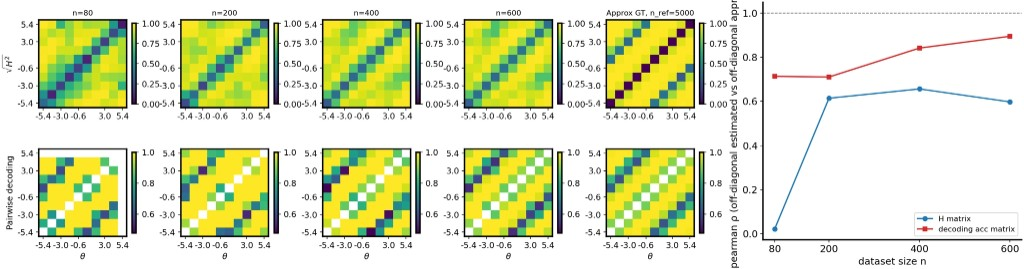
\includegraphics[width=\linewidth]{notes/figures/circular-3d-flow-matching-convergence.png}
  \caption{%
    Flow matching with path integration on the $d=3$ circular (cosine Gaussian $\sqrt{d}$) toy.
    Top row: estimated $\sqrt{H^2}$ RDMs; bottom row: pairwise decoding matrices; columns are training sizes $n$ and an approximate ground truth from a large reference draw.
    Right: Spearman correlation between off-diagonal entries of each estimated matrix and the corresponding approximate ground truth, as a function of~$n$ (Hellinger in blue, decoding in red).}
  \label{fig:circular_3d_flow_matching}
\end{figure}

This behavior is expected in hindsight: turning a learned velocity into a score and integrating along $\theta$ is an indirect route when the stimulus acts through periodic tuning, so approximation error can accumulate.

\subsection{Failure on high-dimensional circular data using exact likelihood computation with flow matching on $\theta$ space and $x$ space}
Flow matching also supports a more direct route: integrate the divergence of the learned velocity along an ODE to obtain a log-density, without converting to a score or integrating a score along~$\theta$.
Let $v_{\phi}$ denote the learned velocity field on observation space.
Then the density carried along the flow obeys
\begin{equation}
  \label{eq:x-ode-inst}
  \frac{\mathrm{d}}{\mathrm{d}t}\log p_t(x_t \mid \theta)
  = - \nabla_{x_t}\!\cdot v_{\phi}(x_t,t\mid\theta) \quad \text{for } x_t \in \mathbb{R}^{d},
\end{equation}
and integrating in time gives the endpoint log-likelihood
\begin{equation}
  \label{eq:x-ode-loglik}
  \log p(x_1\mid\theta)
  =
  \log p_0(x_0)
  -
  \int_0^1 \bigl(\nabla_{x_t}\!\cdot v_{\phi}\bigr)(x_t,t\mid\theta)\,\mathrm{d}t,
\end{equation}
along the trajectory of $\frac{\mathrm{d}}{\mathrm{d}t}x_t = v_{\phi}(x_t,t\mid\theta)$, with $\log p_0$ a standard Gaussian on $\mathbb{R}^d$ at $t=0$.
One may evaluate $\log p(x\mid\theta)$ either by the $x$-space construction in the next paragraph (``$x$-likelihood''), or by the $\theta$-field construction after it (``$\theta$-likelihood'').

\paragraph{$x$-likelihood.}
Here the setup is the most direct: fit \emph{one} conditional flow-matching model on observation space with $\frac{\mathrm{d}}{\mathrm{d}t}x_t = v_{\phi}(x_t,t\mid\theta)$, where $\theta$ is fixed when training and at evaluation time.
For each stimulus value $\theta_j$ and each observation $x_i$, run the ODE likelihood in \eqref{eq:x-ode-inst}--\eqref{eq:x-ode-loglik} with that $\theta_j$ to obtain $\log p(x_i\mid\theta_j)$.
There is no separate prior flow on $\theta$ and no Bayes step: the matrix with entries $C_{ij}=\log p(x_i\mid\theta_j)$ already targets the conditional log-likelihoods needed downstream (with the usual $\Delta L$ diagonal centering applied in the same way as for other $C$~matrices in this project).

\paragraph{$\theta$-likelihood.}
The idea is to run the same likelihood formula on the \emph{stimulus} $\theta$ instead of on~$x$, using two separate flow fits.
The first model ignores the observation and follows $\frac{\mathrm{d}}{\mathrm{d}t}\theta_t = v_{\mathrm{prior}}(\theta_t,t)$; it supplies the prior density $\log p(\theta)$.
The second model conditions on a fixed~$x$ and follows $\frac{\mathrm{d}}{\mathrm{d}t}\theta_t = v_{\mathrm{post}}(\theta_t,t\mid x)$; it supplies $\log p(\theta\mid x)$.
In both cases the endpoint log-density is
\begin{equation}
  \label{eq:theta-ode-loglik}
  \log p(\theta_1)
  =
  \log p_0(\theta_0)
  -
  \int_0^1 \frac{\partial v}{\partial \theta}(\theta_t,t)\,\mathrm{d}t,
\end{equation}
where $\theta_t$ solves the ODE for the active field, $v$ is either $v_{\mathrm{prior}}$ or $v_{\mathrm{post}}(\cdot\mid x)$, and $\log p_0(\theta_0)= -\tfrac{1}{2}\bigl(\theta_0^2 + \log(2\pi)\bigr)$ for a standard normal base on~$\mathbb{R}$.
Subtracting the prior evaluation from the posterior evaluation at the same~$\theta$ yields $\log p(\theta\mid x)-\log p(\theta)$, which Bayes' rule rewrites as $\log p(x\mid\theta)-\log p(x)$.
For a fixed observation~$x_i$, that missing term is the same for every candidate~$\theta_j$ in a row of the pairwise matrix $C_{ij}=\log p(\theta_j\mid x_i)-\log p(\theta_j)$.
The subsequent $\Delta L$ step removes such row-wise constants, so the contrasts line up with differences in $\log p(x_i\mid\theta_j)$.

\paragraph{Fourier features for $\theta$ in the velocity networks.}
Besides choosing whether likelihoods are accumulated in $x$-space or in $\theta$-space, one can change how $\theta$ is presented to the velocity network.
The default is to concatenate the raw scalar $\theta$ (together with time and, depending on the field, $x$ or other inputs) as inputs to a standard multilayer architecture.
An alternative is a \emph{Fourier-feature} parameterization: map $\theta$ to a vector that may include a constant term, the identity term $\theta$, and, for harmonics $k=1,\ldots,K$ and a fixed angular scale $\omega>0$, the pairs $\sin(k\omega\theta)$ and $\cos(k\omega\theta)$, then pass that vector through the same style of network.
This makes periodic structure in $\theta$ easier to represent and is available for both posterior and prior $\theta$-flows, and analogously for the conditional $x$-flow where $\theta$ enters only as a conditioning variable; the harmonic count~$K$ and~$\omega$ are part of the experimental design alongside architecture width and depth.

\subsection{Failure of methods on high-dimensional circular data: results}

Figure~\ref{fig:precision_decoding_matrix_convergence}. I tried also using Spearman correlation, does work.

\begin{figure}[htbp]
  \centering
  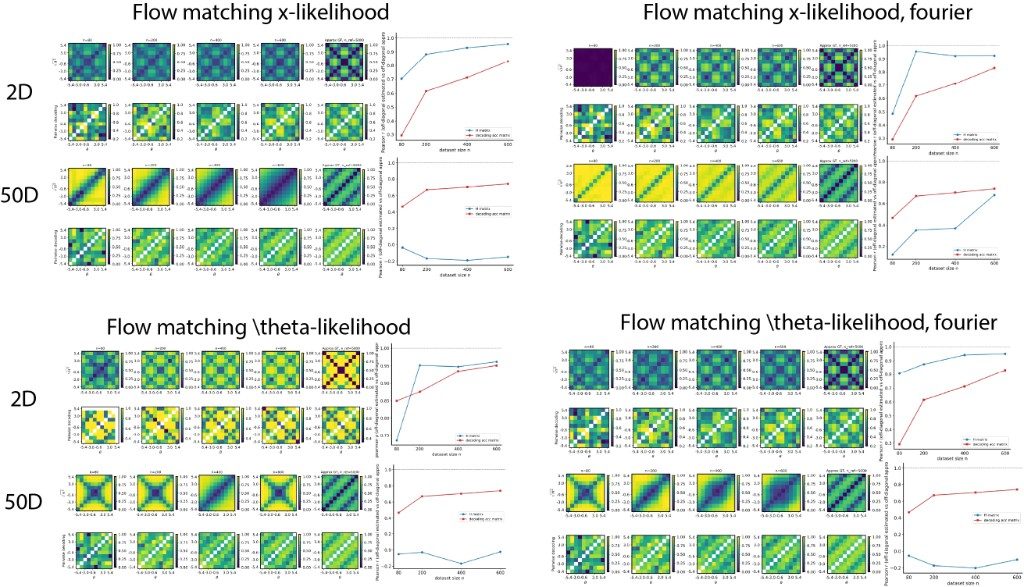
\includegraphics[width=\linewidth]{notes/figures/precision-decoding-matrix-convergence.png}
  \caption{%
    Flow-matching likelihoods: $x$-likelihood (top left), $x$-likelihood with Fourier features on~$\theta$ (top right), $\theta$-likelihood (bottom left), $\theta$-likelihood with Fourier features (bottom right).
    Within each panel, $d=2$ then $d=50$; for each~$d$, top row $\sqrt{\Sigma^{-1}}$--style matrix, bottom row Pearson decoding matrices, columns $n\in\{80,200,400,600\}$ and an approximate ground truth ($n_{\mathrm{ref}}=5000$).
    Side plots: Pearson~$r$ (diagonal of estimate versus off-diagonal match to the reference) versus~$n$ for the $H$/precision matrix (blue) and the decoding-accuracy matrix (red).}
  \label{fig:precision_decoding_matrix_convergence}
\end{figure}

In fact, even increasing the number of data the flow matching method still does not work well, I need to check it.